\chapter{Analysis of Opportunities Enabled by the Data}
\label{cha:high-level-problems}

This chapter describes three interesting high-level problems enabled by the data from the provided dataset.


\section{Improved Bus Stop Detection Algorithm}

The first high-level problem is the problem with inaccurate bus stop detections.
This causes the system to occasionally miss bus stops, which results in faulty or incomplete journeys.
Incomplete journeys require more pre-processing to be done in order to use the data.
Another problem with the existing bus stop detection algorithm is that bus stop coordinates are pre-determined, meaning that they do not always represent the actual bus stop.
This introduces an overhead to the system, where bus stop coordinates need to be updated in order to continue to provide accurate detection of bus stops.

\begin{figure}[ht!]
    \centering
    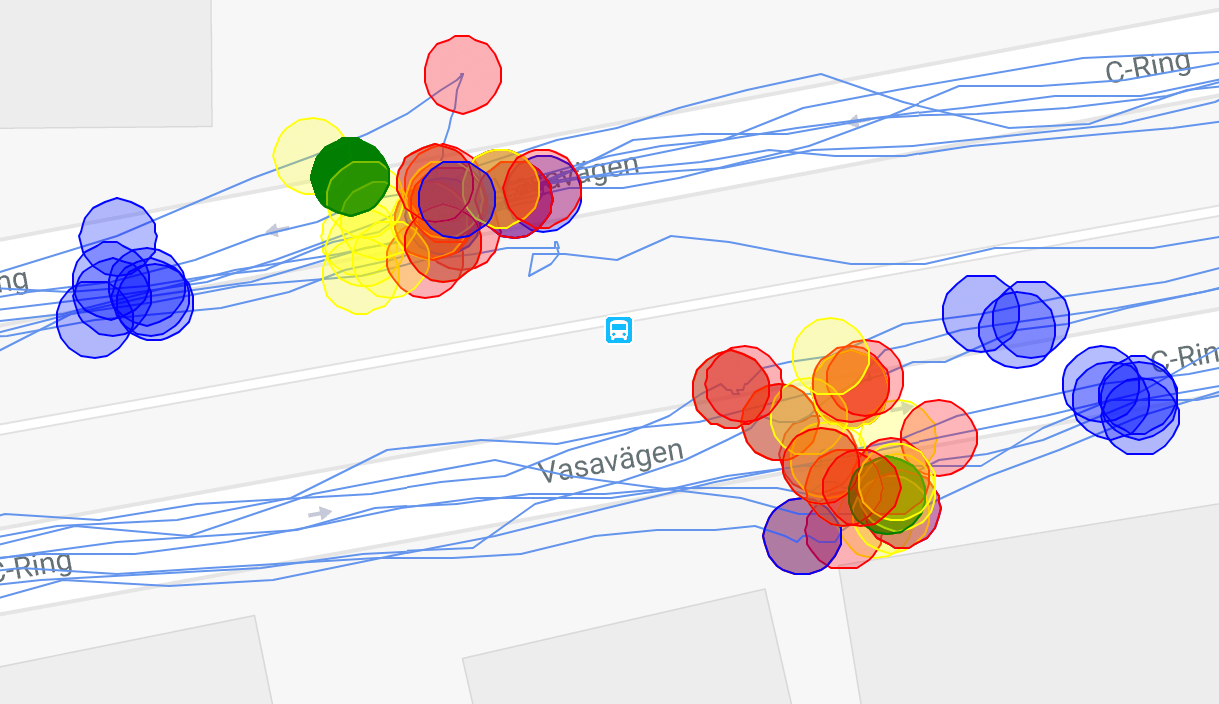
\includegraphics[width=0.9\textwidth]{figures/bus_stops}
    \caption{Output from the Bus Stop Detection Algorithm from the "Internal Analysis" component.
    The green circle are the pre-determined coordinates for the bus stop.
    The bus stop shown has two modes, depending on if the bus travels west (top road) or east (bottom road).
    The red and yellow clusters are the GPS positions of the bus when it arrives to the bus stop.
    The blue clusters are the GPS positions of the buses departing from the bus stop.
    }
    \label{fig:bus-stop-clusters}
\end{figure}

Figure \ref{fig:bus-stop-clusters} shows the results from the existing Bus Stop Detection Algorithm of the "Internal Analysis" component.
Each bus produces seven GPS coordinates for each bus stop: one blue, two red, two yellow, and one green.
The green GPS coordinate is always the same between all buses for each bus stop; it is the pre-determined coordinate for the bus stop.
The blue GPS coordinate is the position of the bus when it departures from the bus stop (the last positional update within a pre-determined radius of the bus stop).
The red and yellow coordinates are the positions of the buses when the system determines that they have arrived (stopped) at the bus stop.
Due to lacking documentation, the difference between the red and yellow coordinates are unclear as they are occasionally identical, but not always (as shown in the figure).
The existing bus stop detection algorithm thus checks within a pre-determined radius around the green GPS coordinate for updates from buses.
When the first positional update from the bus is received, the system tracks the bus and waits for it to stop.
Upon stopping, the bus is determined to have arrived at the bus stop.
When the bus starts again, the system continues to track it and reports when the bus has left the radius of the bus stop.
The blue GPS coordinate shows where this happens. 


\section{GPS Variation Estimation}

The main component of the dataset is the GPS positional update events from the vehicles.
They contribute to roughly 96\% of the events in the data, as shown by Figure \ref{fig:types-barplot} in Section \ref{sec:data-structure}.
An interesting high-level problem is thus the estimation of the variance in the GPS positions.
The hypotheses are that the GPS positions vary depending on:
\begin{enumerate}
    \item \textit{Environment (Spatial Locality):} 
    The surrounding environment impacts the visibility of GPS satellites. \todo{source?}
    For example, in an environment with a lot of reflections and obstacles, the precision of the GPS position will decrease.
    On the other hand, in open fields the precision will increase, as there are fewer obstacles blocking the GPS satellite signals.
    The environment can vary between different road segments, but also inside one road segment, e.g., a road can be partly covered by houses or trees.
    The variance could either be seen as continuous, where each point on the journey has its own variance, or as road segments, where each road segment has its own variance.
    In the continuous case, neighbouring pairs of points would be connected and thus exhibit more similar variance, depending on the distance between the points (granularity) in a journey.
    In the case of road segments, different segments would exhibit a, potentially, larger difference in variance.
    
    Road segments could either be created geographically, e.g., a segment is the road between two bus stops or between crossings, or contextually from the output of the continuous case.
    A geographical road segmentation would most likely get a higher average variance, as the environment could change within the segment.
    The contextual segmentation would look at sequences of points in the journey, and group the sequential points which exhibit similar variance.
    The result would potentially be segments where the inherent variance of each segment is lower than between different segments.

    Figure \ref{fig:gps-variation} illustrates how the GPS variance can differ for different road segments.
    In the shown scenario, the difference between geographical segmentation between crossings and contextual segmentation would be minor, as the variance seems to be similar for a given road segment.
    However, the difference would be major if the geographical segmentation was done between bus stops.
    The number of road segments would be higher in the crossing-geographical approach than in the contextual approach, as, for example, "Järnvägsgatan" have many crossings but exhibit similar variance. 
    

    \item \textit{GPS Sensor Calibration:}
    Each bus has its own GPS sensor, where different buses could have different models with their own calibrations.
    In the general case the different GPS sensors show small variance due to different calibrations.
    However, occasionally they can vary, e.g., by some constant factor, as shown in Figure \ref{fig:gps-sensor-calibration}.
    The single orange-coloured bus journey seems to have a constant offset compared to the rest of the journeys for that particular bus line.
    The shown scenario is quite extreme, as the offset is large enough to cause problems with the Bus Stop Detection Algorithm in the "Internal Analysis" component.
    No bus stops are detected in this particular scenario.
    These extreme situations can thus be detected by combining the positional events with the bus stop events.
    However, differences in calibrations which yield smaller offsets cannot be detected with this combining approach.


    \item \textit{Time:}
    The timestamp of the position events affects the precision of the GPS sensor.
    At a single given point of the journey the precision could vary depending on the positions of satellites and the amount of satellites visible.
    The hypothesis is that there is a constant bias to the GPS positions depending on the timestamp.
    The positions of the satellites thus cause a small offset to occur in the GPS position.
    This parameter probably has some periodicity, which could be fitted using a Gaussian Process with a periodical kernel.
    
\end{enumerate} 


\begin{figure}[ht!]
    \centering
    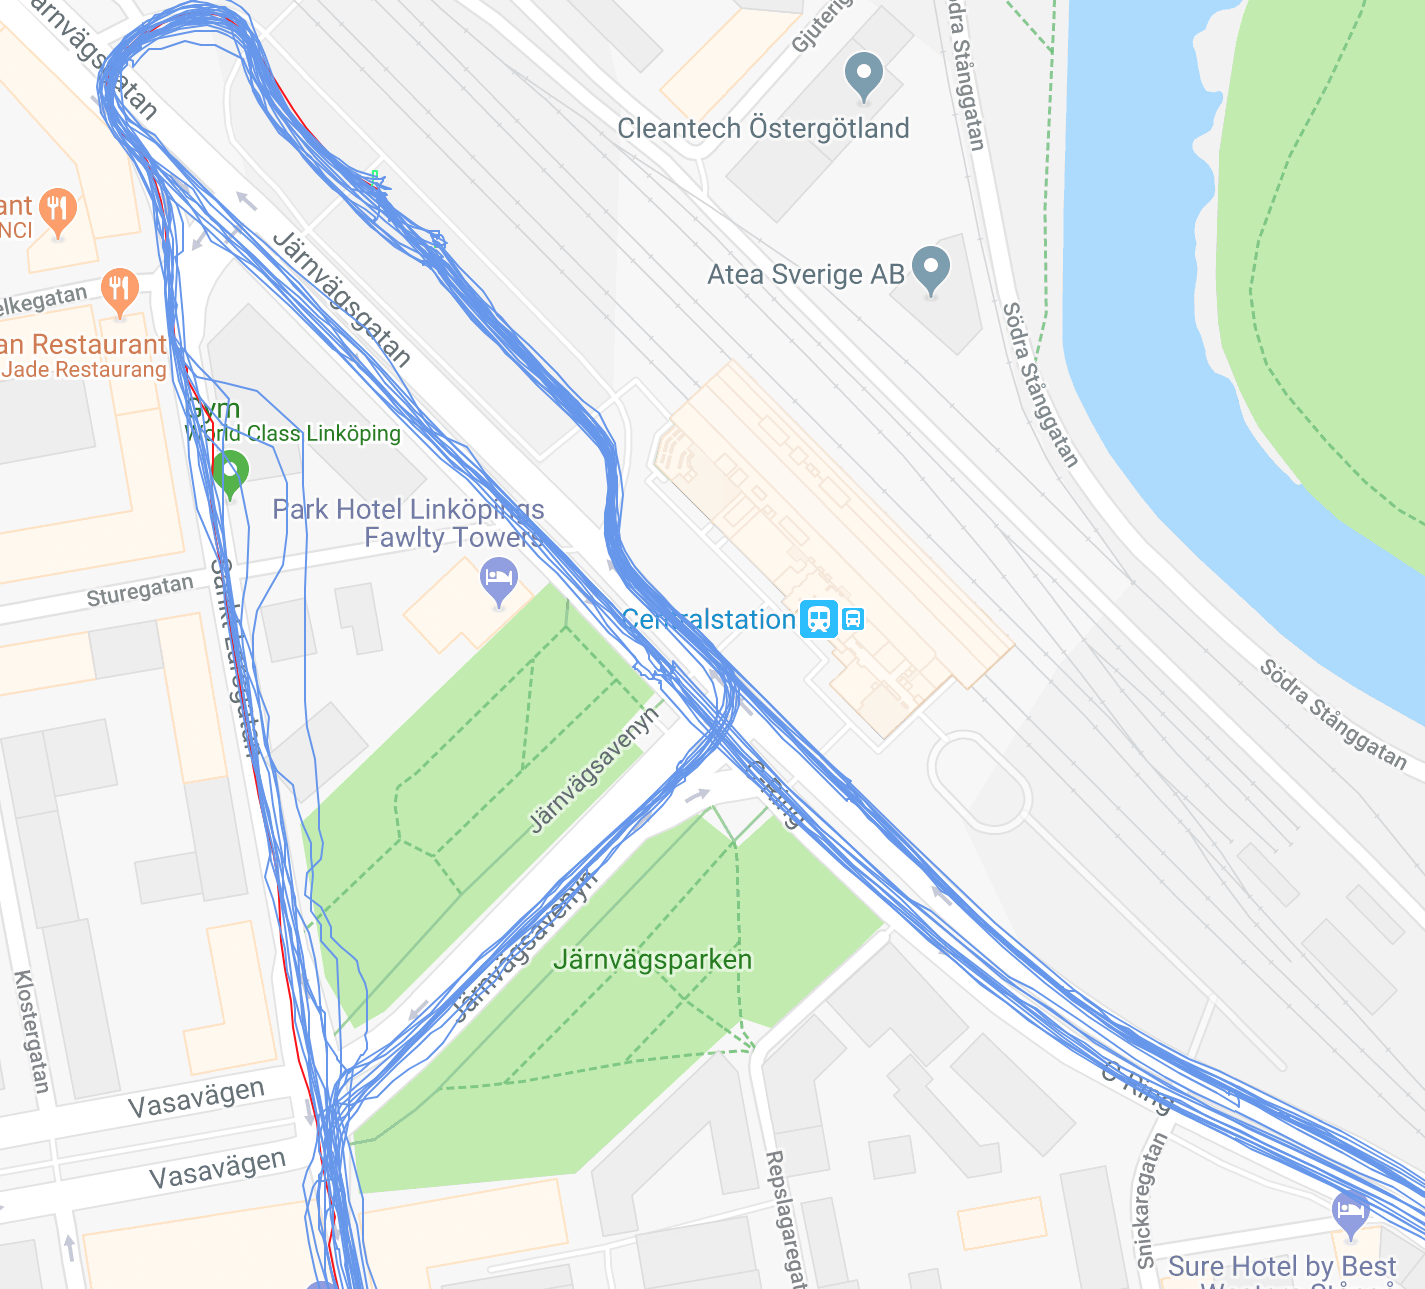
\includegraphics[width=0.9\textwidth]{figures/gps_variation}
    \caption{Visualisation of multiple journeys by different buses in the same area.
    Each blue line is a journey in the "Started" state.
    The variance differs between different road segments, as shown around "World Class Linköping" compared to "Järnvägsgatan".}
    \label{fig:gps-variation}
\end{figure}

\begin{figure}[ht!]
    \centering
    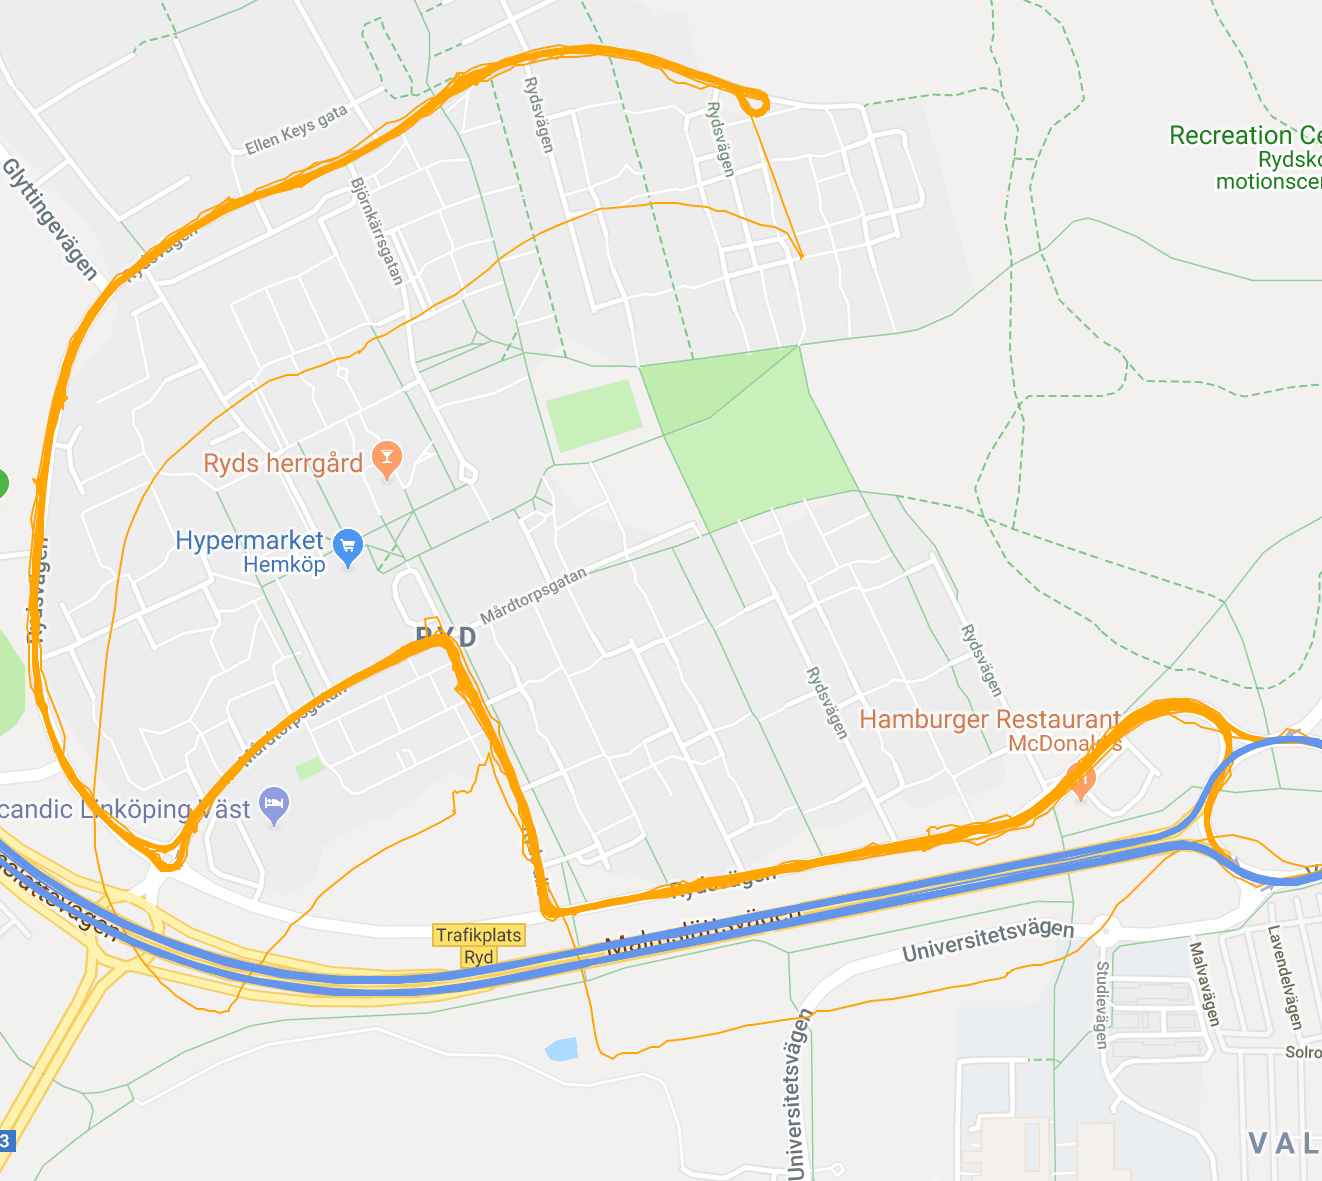
\includegraphics[width=0.9\textwidth]{figures/gps_sensor_calibration}
    \caption{Illustrates the case of a poorly calibrated GPS sensor on an individual bus.
    The orange lines creating the thicker line are all the other journeys for the same bus line, but done by other buses.
    The thin orange line is one bus with an extremely poorly calibrated GPS sensor.
    It seems to have a constant offset compared to the rest.
    This real-world scenario shows that the calibration of GPS sensors is important in order to produce useful data.}
    \label{fig:gps-sensor-calibration}
\end{figure}

\subsection{Road Segment Data}
Google Maps provides a Roads API\footnote{https://developers.google.com/maps/documentation/roads/intro} to map GPS coordinates to the closest road segment.
The road segments could, for example, be used to create a model calculating the orthogonal variance of GPS coordinates with respect to the road segments.
\todo{Bild?}
However, the variance of GPS positions does not only occur orthogonal to a given road segment. \todo{Vart vill jag komma med det här?} 

Manual inspection of journeys done in the pre-processing step highlights scenarios with discrepancies between roads in Google Maps and actual roads the buses drove.
The Google Maps roads are in these scenarios usually incorrectly drawn or has missing roads or buildings.
Figure \ref{fig:gps-map-problem} shows such a real-world example.
The discrepancies would cause problems if used naïvely together with the Google Maps Roads API.
These journeys would have to be detected and either handled or ignored.
The detection could be done by looking at the distances to the closest Google Maps Roads segments.
The distances would roughly be similar for all the journeys, as in Figure \ref{fig:gps-map-problem}.
Since the distances would be roughly similar they could be averaged and interpreted as a bias to the roads.
Applying the bias-interpretation methodology would result in a more generalised model using the Google Maps Roads API.
Ignoring the journeys with discrepancies could also be seen as feasible, given that the occurrence is rare.
Before using the simpler approach of ignoring journeys with discrepancies, a deeper analysis needs to be conducted.

\begin{figure}[ht!]
    \centering
    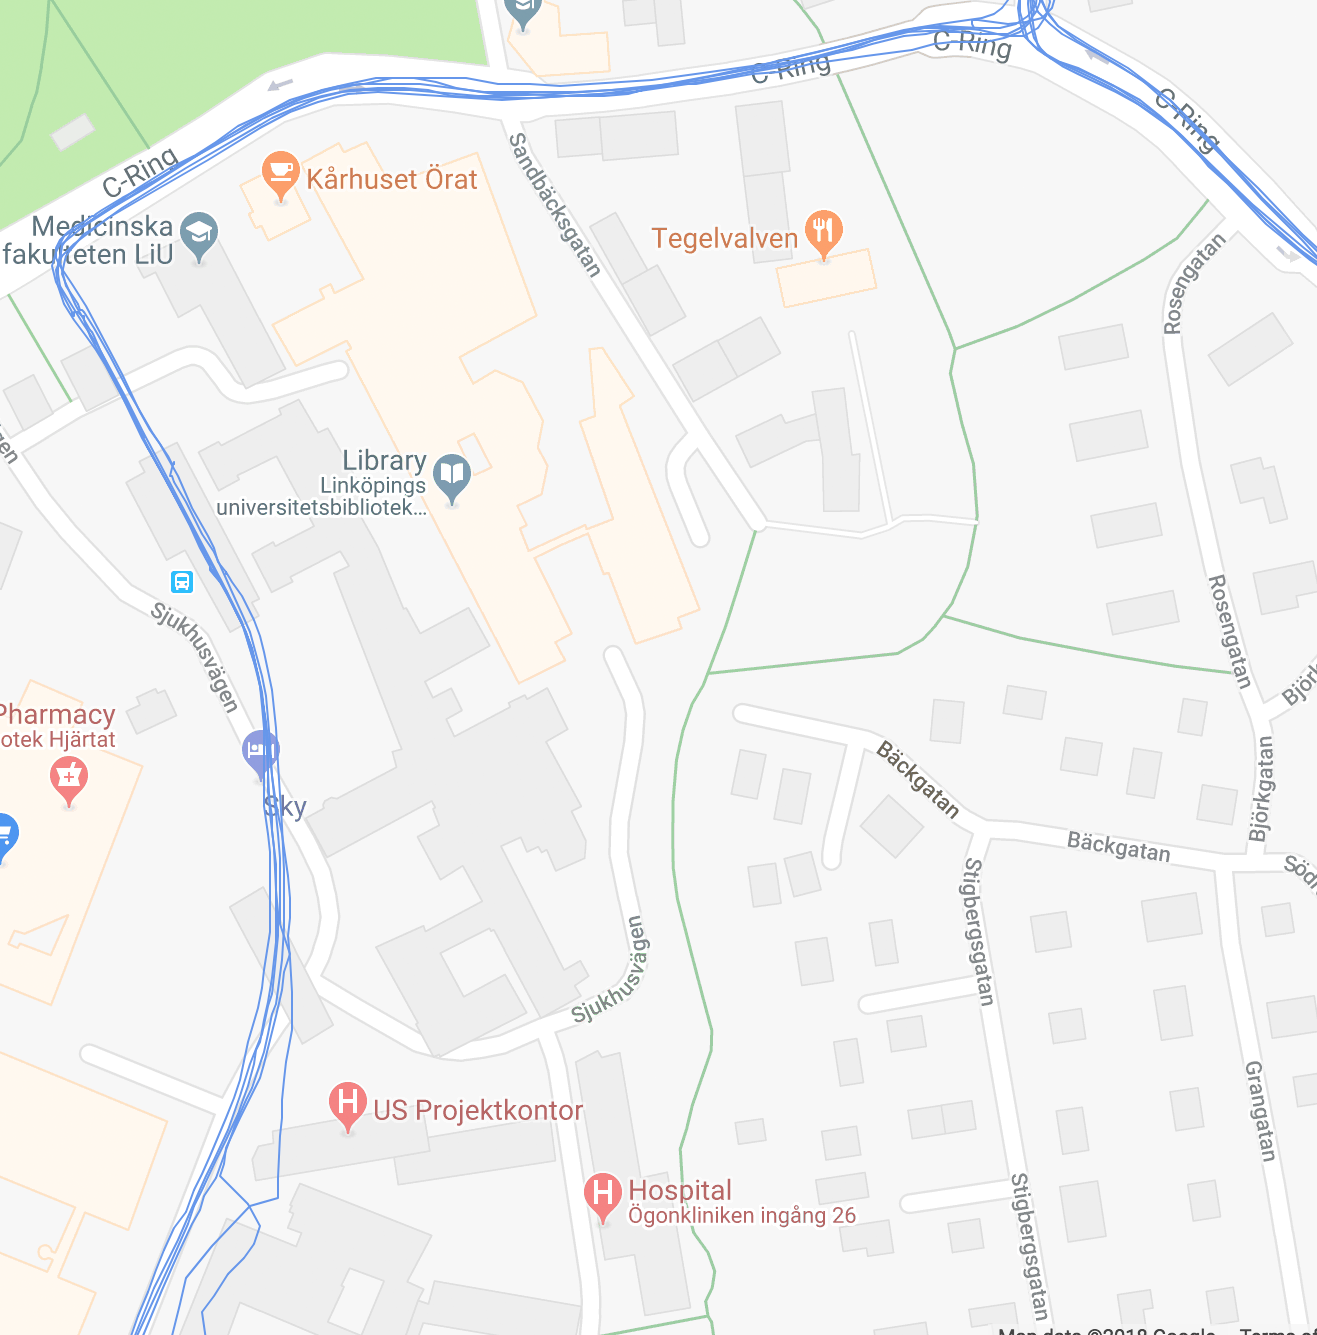
\includegraphics[width=0.9\textwidth]{figures/gps_map_problem}
    \caption{Real-world example of multiple buses driving on a road not correctly modelled by Google Maps.
    For example, at "Sjukhusvägen" the buses are driving through a building according to Google Maps.
    In this particular scenario the area has received major road re-structuring and renovation.
    The Google Maps representation is thus likely outdated.}
    \label{fig:gps-map-problem}
\end{figure}

\section{Trajectory Forecasting} \label{sec:problems-trajectory-forecasting}
Trajectory Forecasting is the process of determining when a bus arrives at a given bus stop.
The existing Trajectory Forecasting is based purely on long-time historical data.
It provides a single timestamp when it predicts the bus to arrive at a certain bus stop.

